\documentclass[11pt]{article}

%Don't change any thing before \begin{document}
%In fact if you use sth fancy, you might need
%to add more packages, or macros.


\usepackage{../EllioStyle}



\begin{document}
\date{March 12, 2020}
\ShortHeadings{Computer Science Theory: Assignment~3}{Elliott Pryor}
\title{CSCI 338: Assignment~3~(6 points)}

\author{Elliott Pryor}


\maketitle

%When writing up your solution, comment out the following until you reach Problem 1.
\noindent
This assignment is due on {\bf Tuesday, March 10, 11:30pm}. It is strongly
encouraged that you use Latex to generate a single pdf file and upload it
under {\em Assignment 3} on D2L. But there will NOT be a penalty for not
using Latex (to finish the assignment). This is {\bf not} a group-assignment,
so you must finish the assignment by yourself.

\section*{Problem 1}

\noindent
Design context-free grammars for the following languages

(1.1) $A=\{a^nb^m|n\neq 2m\}$.

\begin{itemize}
\item $S = aaSb | A | aB | B$
\item $A = aA | a$
\item $B = bB | b$
\end{itemize}


(1.2) $B=\{a^ib^jc^k|i,j,k\geq 0$ and either $i=j$ or $j=k\}$.

\begin{itemize}
\item $S = XC | AY$
\item $A = aA | \epsilon$
\item $C = cC | \epsilon$
\item $X = aXb | \epsilon$
\item $Y = bXc | \epsilon$

\end{itemize}

(1.3) $C=\{a^nb^m|n=3m\}$.

\begin{itemize}
\item $S = aaaSb | \epsilon$

\end{itemize}

(1.4) $D=\{a^nb^m|n\leq m+3\}$.

\begin{itemize}
\item $S = aSb | Sb | A $
\item $A = aaa | aa | a | \epsilon$

\end{itemize}



\newpage
\section*{Problem 2}

\noindent
Decide whether the following grammar is ambiguous.
\newline

$S\rightarrow AB|aaB$

$A\rightarrow a|Aa$

$B\rightarrow b$


\begin{table}[h!]
\begin{tabular}{c | c}
Derivation 1 & Derivation 2\\
\hline
S & S\\
AB & aaB\\
AaB & aab\\
aaB & \\
aab & \\
\end{tabular}

\end{table}


There are multiple ways to generate the string ``aab'' with this grammar, so \textbf{yes} the grammar is ambiguous.

\newpage
\section*{Problem 3}

\noindent
Convert the following CFG G to an equivalent PDA.

$R\rightarrow XRX|S$

$S\rightarrow aTb|bTa$

$T\rightarrow XTX|X|\epsilon$

$X\rightarrow a|b$

\begin{figure}[h!]
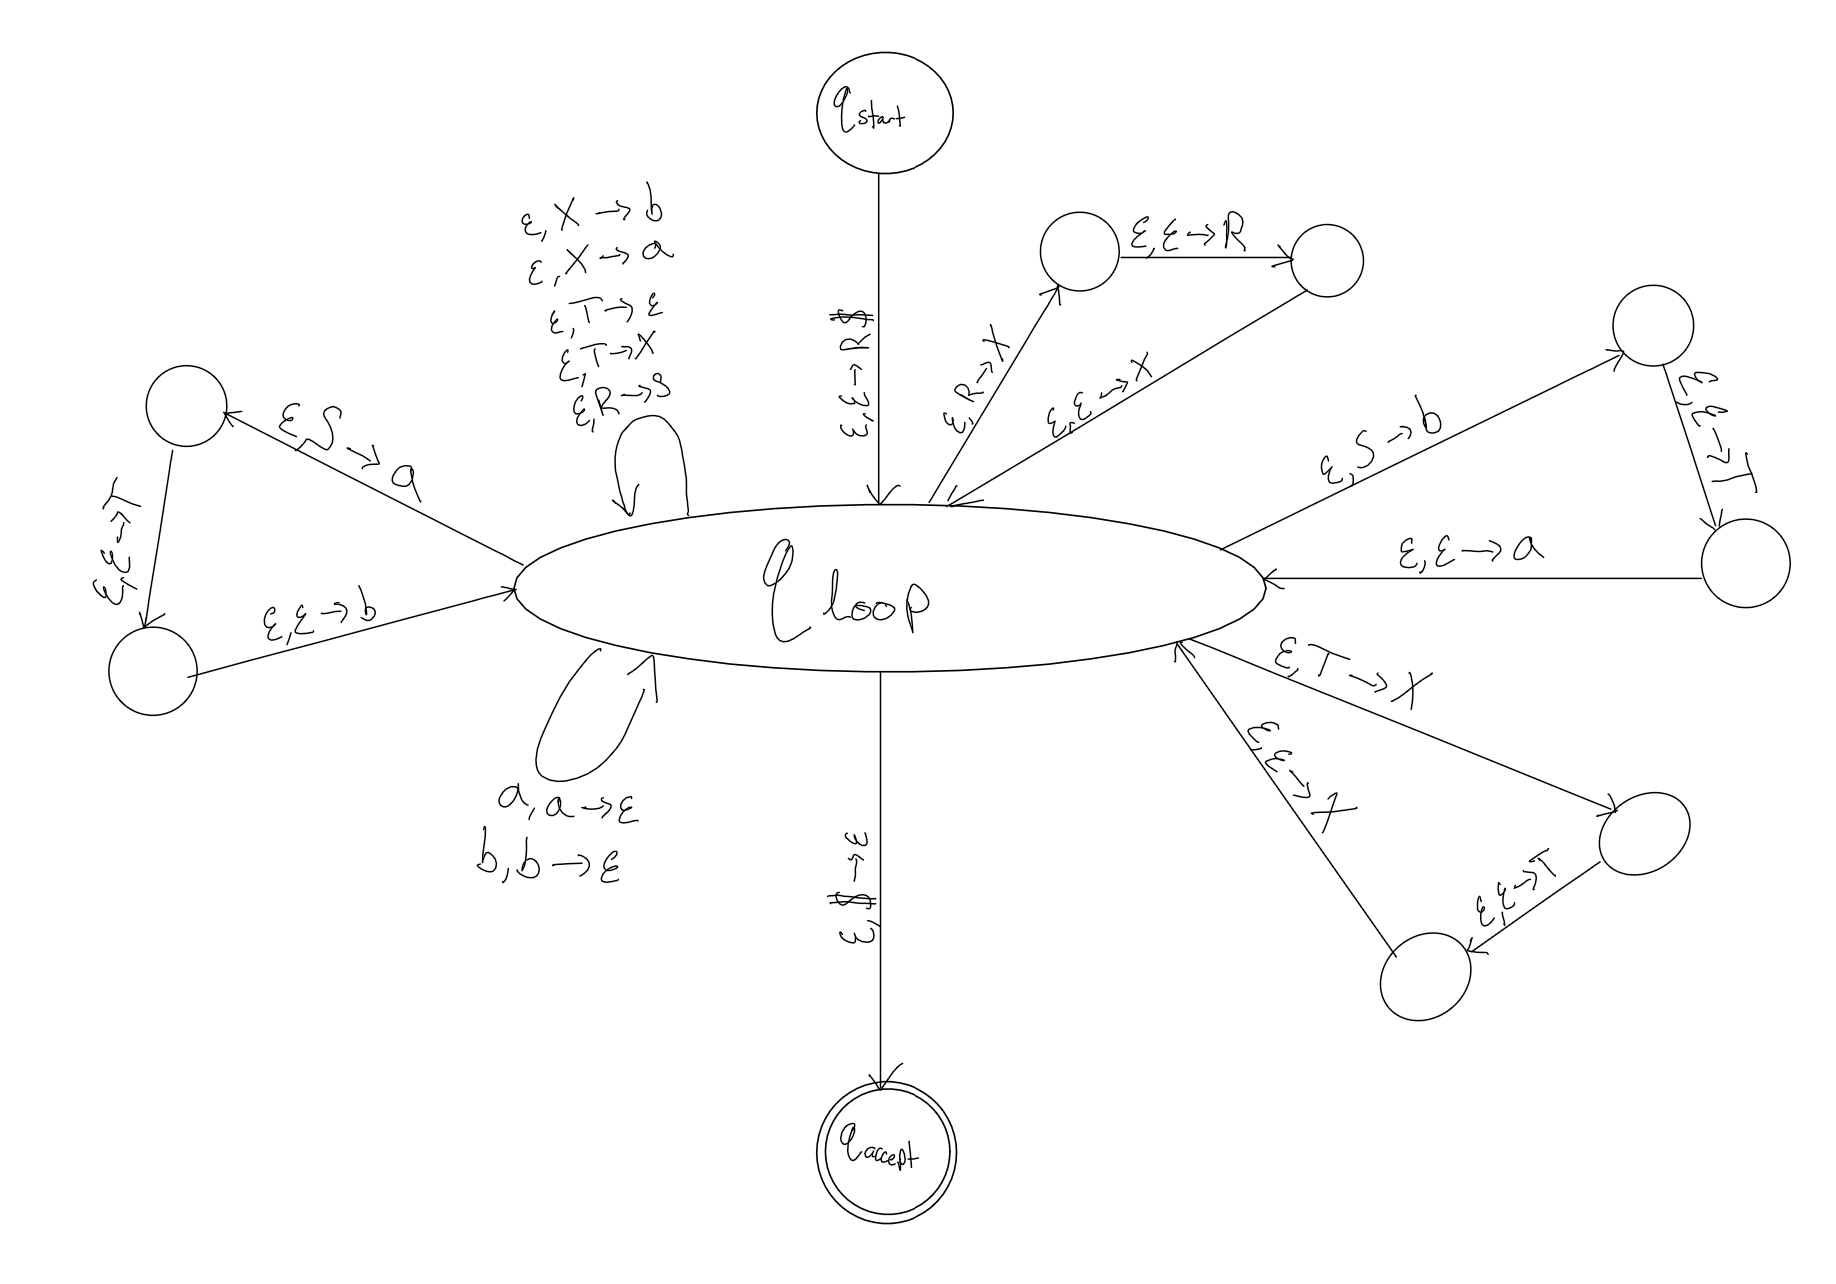
\includegraphics[scale=1]{problem3.png} 
\caption{Solution to Problem 3}
\end{figure}



\newpage
\section*{Problem 4}

\noindent
Let $G=(V,\Sigma,R,S)$ be the following grammar. $V=\{S,T,U\}$;
$\Sigma=\{0,\#\}$; and $R$ is the set of rules:

$S\rightarrow TT|U$

$T\rightarrow 0T|T0|\#$

$U\rightarrow 0U00|\#$

\noindent
\textbf{(4.1) Describe $L(G)$ in English.}
\newline

$L(G)$ has two $\#$'s within a list of zeros. Or L(G) a single $\#$ one third of the way through a list of zeros with a multiple of three length. Ie. it has a list of $n$ zeros, a single $\#$ then a list of $2n$ zeros.

\noindent
\textbf{(4.2) Prove that $L(G)$ is not regular.}

\begin{proof} By Contradiction.

Assume that $L(G)$ is regular. Then we pick $S= 0^p \# 0^{2p}$

By the pumping lemma, $S$ can be decomposed into $xyz$ s.t.

\begin{enumerate}[(1)]
\item $xy^iz \in A$ for $i \geq 0$
\item $|y| > 0$
\item $|xy| \leq p$ 
\end{enumerate}

Let $i = |y|$, then by (2) $i = |y| > 0$, and by (3) $|xy| \leq p$ so $y$ must consist of only zeros. We pump up $xy^2z = 0^{p + i} \# 0^{2p} \notin L$ because we increased the number of zeros before the $\#$ without changing those after it, so $2(p+i) \neq 2p$.

A contradiction of the pumping lemma, so $L$ must not be regular.

\end{proof}

\newpage
\section*{Problem 5}

\noindent
Convert the following CFG into an equivalent CFG in Chomsky Normal Form

$A\rightarrow BAB|B|\epsilon$

$B\rightarrow 00|\epsilon$
\hline


$S_0 \rightarrow BC | AB | BA | BB | XX$\\
$A \rightarrow BC | AB | BA | BB | XX$\\
$B \rightarrow XX$\\
$C \rightarrow AB$\\
$X \rightarrow 0$\\


\begin{figure}[h!]
	\centering
	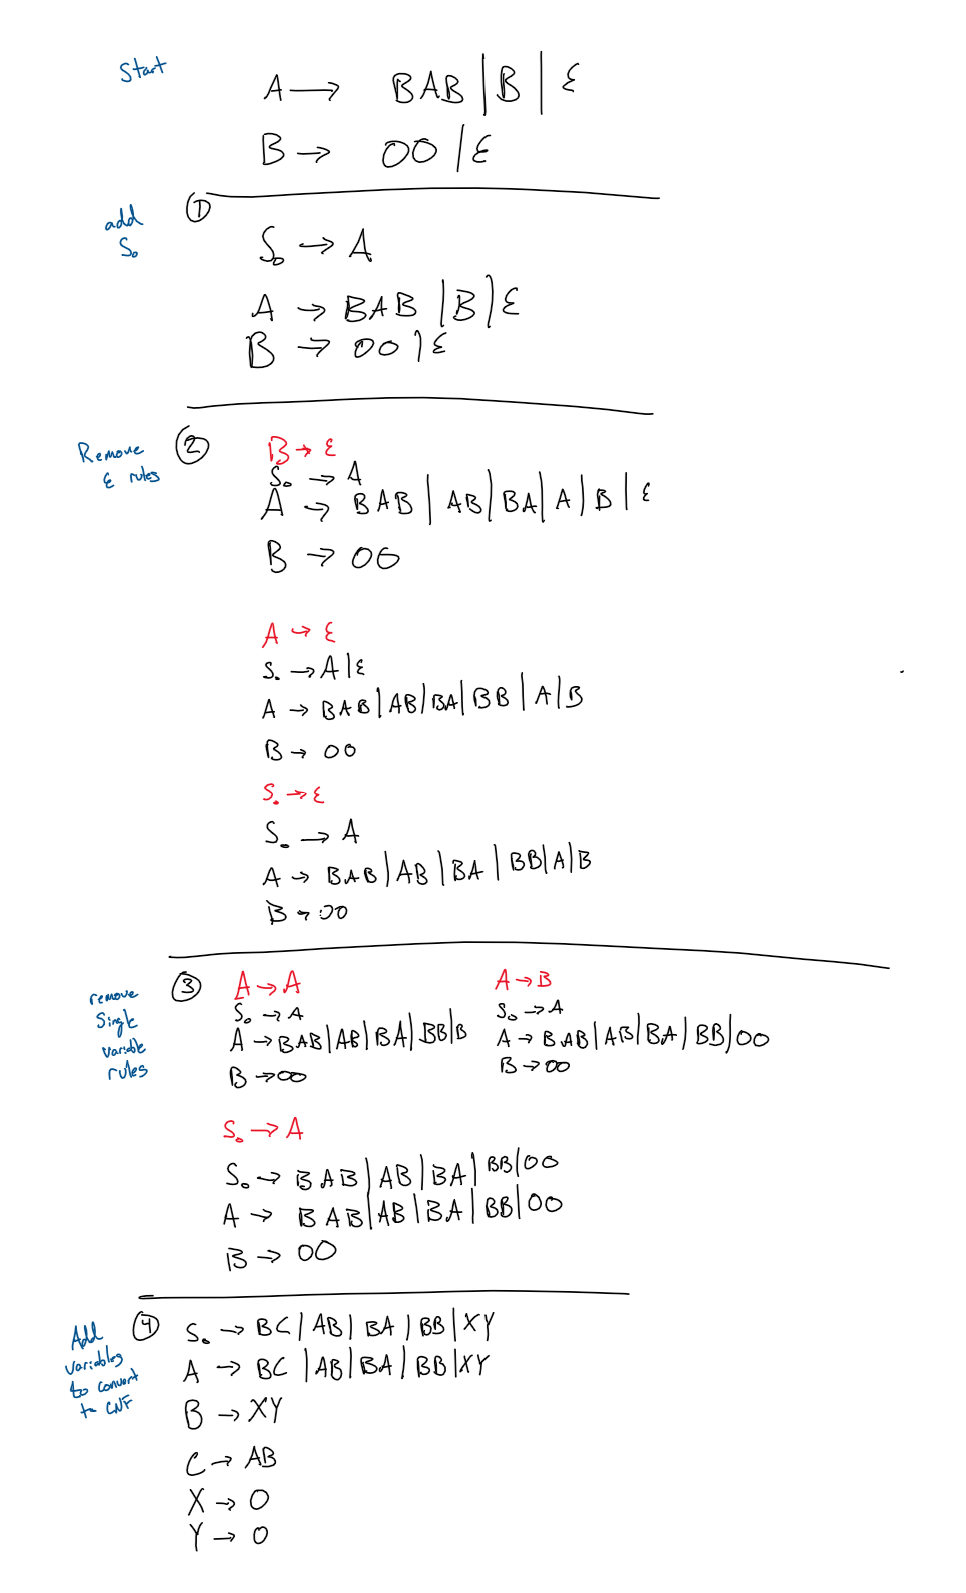
\includegraphics[scale=0.9]{problem5.png} 
	\caption{Work for Problem 5}
\end{figure}

\newpage
\section*{Problem 6}

\noindent
Using pumping lemma to prove that the following languages are not
context-free.

\textbf{(6.1) $L=\{a^nb^jc^k|k=nj\}$.}
\newline

\begin{proof} By Contradiction

Assume that $L$ is regular. Then pick $S = a^p b^p c^{p^2}$ where $p$ is the pumping length. Then by the pumping lemma $S$ can be decomposed into $S = uvxyz$ st.

\begin{enumerate}[(1)]

 \item $uv^ixy^iz \in L$ for $i \geq 0$
 \item $|vy| > 0$
 \item $|vxy| \leq p$

\end{enumerate}

We examine three cases:
\begin{enumerate}
	\item $vxy$ contains $b$'s and $c$'s. Pumping up, $uv^2xy^2z$ is of the form $a^p b^{p + i} c^{p^2 + j}$. Then $p(p+i) = p^2 + ip > p^2 + j$ because $i > 0$ therefore $j < p$ by (3). Therefore $uv^2 x y^2 z \notin L$
	\item $vxy$ contains no $c$'s. Then, we pump up $uv^2 x y^2 z \notin L$ by (2), $|vy| > 0$ so there is more $a$'s or $b$'s without changing the number of $c$'s. 
	\item $vxy$ contains only $c$'s. Then, we pump up $uv^2 x y^2 z \notin L$ by (2), $|vy| > 0$ so there is more $c$'s without changing the number of $a$'s or $b$'s.

\end{enumerate}

Thus a contradiction in all cases, so $L$ is not regular.

\end{proof}






\textbf{(6.2) $L=\{a^nb^j|n\geq (j-1)^3\}$.}
\newline

\begin{proof} By Contradiction

Assume that $L$ is regular. Then pick $S = a^{(p-1)^3} b^p$ where $p$ is the pumping length. Then by the pumping lemma $S$ can be decomposed into $S = uvxyz$ st.

\begin{enumerate}[(1)]

 \item $uv^ixy^iz \in L$ for $i \geq 0$
 \item $|vy| > 0$
 \item $|vxy| \leq p$
\end{enumerate}

We examine three cases:

\begin{enumerate}
  \item $vxy$ consists only of $a$'s. We pump down so $uv^0 x y^0 z = uxz$. By (2) $i = |vy| > 0$, so $uxz$ has the form $a^{(p-1)^3 - i} b^p$, but $(p-1)^3 - i < (p-1)^3$. Therefore $uxz \notin L$.
  \item $vxy$ contains both $a$'s and $b$'s. We pump up, $uv^2xy^2z$ is of the form $a^{(p-1)^3 + i} b^{p + j}$. We know that $j \neq 0$ so $(p + j - 1)^3 \geq p^3$, and $i < p$ by (3). Then $(p-1)^3 + i < (p-1)^3 + 3p^2 - 3p + 1 = p^3$ for $p > 1$. Therefore $(p-1)^3 + i < (p + j - 1)^3$. Therefore $uxz \notin L$
  \item $vxy$ contains only $b$'s. We pump up, $uv^2xy^2z$ is of the form $a^{(p-1)^3}b^{p + i}$. By (2), $i = |vy| > 0$, so we increase the number of $b$'s without altering the number of $a$'s. Then $(p-1)^3 < (p + i - 1)^3$, therefore $uxz \notin L$.
\end{enumerate}

Thus a contradiction in all cases, so $L$ is not regular.

\end{proof}

\end{document}
